\documentclass[tikz,border=8pt]{standalone}
% Shared look for every TikZ diagram. Load with \input{../../tools/tikz-style.tex}
\usepackage[T1]{fontenc}
\usepackage{lmodern}
\renewcommand{\sfdefault}{lmr}  % diagrams use the same serif as the text
\usetikzlibrary{arrows.meta, positioning, shapes.geometric, calc, fit, backgrounds}
\definecolor{cblue}{HTML}{4C78A8}
\definecolor{corange}{HTML}{F58518}
\definecolor{cgreen}{HTML}{54A24B}
\definecolor{cred}{HTML}{E45756}
\definecolor{cpurple}{HTML}{B279A2}
\definecolor{cgrey}{HTML}{6B6B6B}
\tikzset{
  every picture/.style={font=\sffamily, line width=1.2pt},
  box/.style={draw=#1, fill=#1!12, rounded corners=4pt, align=center, inner sep=7pt, minimum height=1.1cm},
  box/.default=cgrey,
  arrow/.style={-{Stealth[length=3mm]}, draw=cgrey, line width=1.4pt},
  title/.style={font=\sffamily\bfseries\Large},
  note/.style={font=\sffamily\small, text=cgrey, align=center},
}
\AtBeginDocument{\hyphenpenalty=10000 \exhyphenpenalty=10000}

\usetikzlibrary{matrix}
\begin{document}
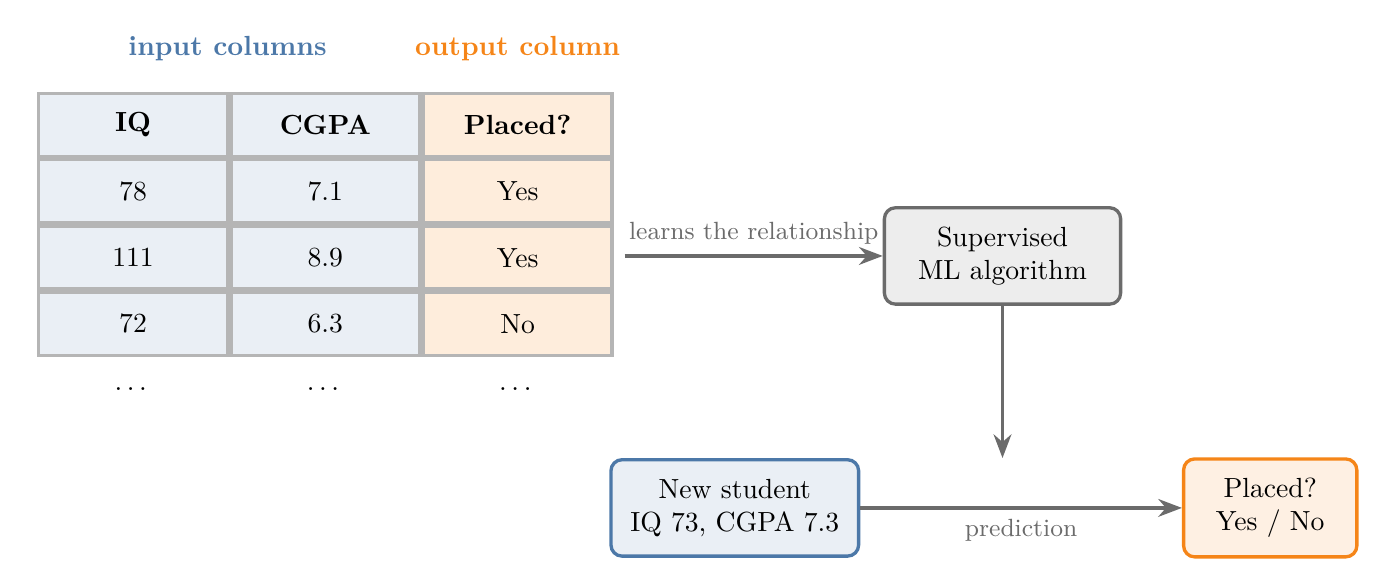
\begin{tikzpicture}
  \matrix (t) [matrix of nodes, nodes={minimum width=2.4cm, minimum height=0.8cm, anchor=center, draw=cgrey!50},
               column 1/.style={nodes={fill=cblue!12}}, column 2/.style={nodes={fill=cblue!12}},
               column 3/.style={nodes={fill=corange!15}}, row 1/.style={nodes={font=\sffamily\bfseries}}]
  {
    IQ  & CGPA & Placed? \\
    78  & 7.1  & Yes \\
    111 & 8.9  & Yes \\
    72  & 6.3  & No  \\
    |[draw=none, fill=none]| \dots & |[draw=none, fill=none]| \dots & |[draw=none, fill=none]| \dots \\
  };
  \node[cblue, font=\sffamily\bfseries, above=0.25cm of t-1-1, xshift=1.2cm] {input columns};
  \node[corange, font=\sffamily\bfseries, above=0.25cm of t-1-3] {output column};
  \node[box=cgrey, minimum width=3cm] (m) at (8.6,0) {Supervised\\ML algorithm};
  \draw[arrow] (t.east) -- node[note, above] {learns the relationship} (m);
  \node[box=cblue, minimum width=2.6cm] (new) at (5.2,-3.2) {New student\\IQ 73, CGPA 7.3};
  \node[box=corange, minimum width=2.2cm] (ans) at (12.0,-3.2) {Placed?\\Yes / No};
  \draw[arrow] (new) -- node[note, below] {prediction} (ans);
  \draw[arrow] (m) -- (m |- new.north);
\end{tikzpicture}
\end{document}
